\newcommand{\sampleio}{%
  \setcounter{samplenum}{0}%
  \includesample{1}%
}


\problemname{Cargo Calibration Protocol}

\begin{wrapfigure}{r}{0.4\textwidth}
  \vspace{-1em}
  \centering
  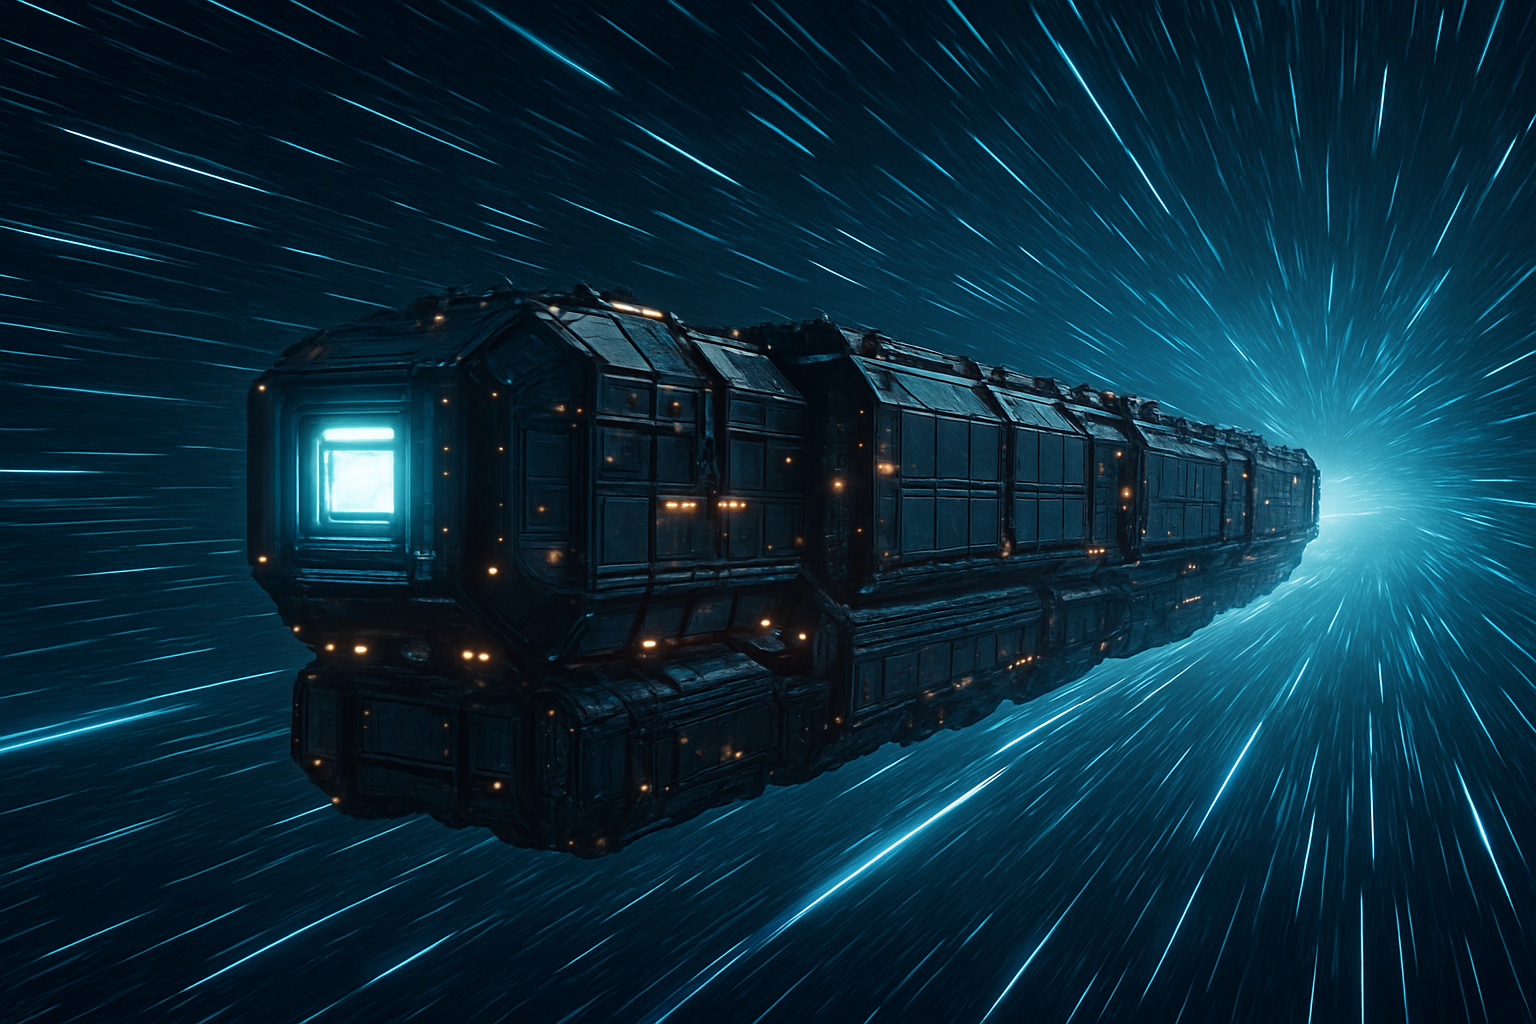
\includegraphics[width=0.4\textwidth]{cargoship.png}
\end{wrapfigure}
\noindent You are an operations engineer aboard the interstellar freighter Orion’s Reach. The ship is preparing for a hyperspace jump, but before that can happen, its cargo loadout must be calibrated carefully.
Each crate on the ship contains modules with varying mass values. Every crate has a specific set of components that could be loaded, each with a defined weight. The ship’s core AI randomly selects one component from each crate to include in the final cargo configuration.
A successful configuration is one where the total cargo weight falls within a safe operational range for the hyperspace jump. Too light or too heavy, and the jump could fail catastrophically.
Your task is to calculate the probability that a random cargo configuration will result in a total weight within the safe bounds.

\section*{Input}

\begin{itemize}
  \item The first line contains three integers:
  n – the number of cargo crates (1 <= n <= 100)
  min and max – the minimum and maximum acceptable total weight for the jump (1 <= min = max <= 1,000)
  \item 
  The following n lines describe each crate:
  First an integer s (1 <= s <= 100), the number of available components for that crate,
  followed by s integers, each representing the weight of one component option
\end{itemize}

\section*{Output}

Print the probability (as a percentage, rounded to two decimal places) that a randomly selected configuration of components results in a total weight between min and max, inclusive.

\noindent Note that a margin of error of ±1\% is acceptable.
